% =========================================================================
% ICDEES 2026 Conference Paper Manuscript (IEEE Format - Revised Version 6)
% Venue: International Conference on Digital Economy and Emerging Societies (ICDEES 2026)
% IEEE Proceedings / IEEE Xplore Indexing
% Formatting: IEEEtran Conference (Double-Blind Review Ready)
% Structure: IMRaD (Introduction, Method, Result, Discussion, Conclusion)
% Target Length: Strictly 6 Pages Maximum (Zero Spillover to Page 7)
% =========================================================================

\documentclass[conference]{IEEEtran}
\IEEEoverridecommandlockouts

% -------------------------------------------------------------------------
% Core Packages & Typographical Optimization
% -------------------------------------------------------------------------
\usepackage{cite}
\usepackage{amsmath,amssymb,amsfonts}
\usepackage{algorithmic}
\usepackage{algorithm}
\usepackage{graphicx}
\usepackage{textcomp}
\usepackage{xcolor}
\usepackage{booktabs}
\usepackage{array}
\usepackage{adjustbox}
\usepackage{url}
\usepackage{microtype}
\usepackage[letterpaper, top=0.72in, bottom=0.92in, left=0.68in, right=0.68in, columnsep=0.24in]{geometry}
\raggedbottom

% -------------------------------------------------------------------------
% Float Spacing & Typographical Compression (Strict 6-Page Guarantee)
% -------------------------------------------------------------------------
\setlength{\textfloatsep}{2.2pt plus 0.5pt minus 0.5pt}
\setlength{\floatsep}{1.8pt plus 0.5pt minus 0.5pt}
\setlength{\intextsep}{1.8pt plus 0.5pt minus 0.5pt}
\setlength{\dbltextfloatsep}{2.2pt plus 0.5pt minus 0.5pt}
\setlength{\dblfloatsep}{1.8pt plus 0.5pt minus 0.5pt}
\setlength{\abovecaptionskip}{1.8pt plus 0.5pt minus 0.5pt}
\setlength{\belowcaptionskip}{0.8pt plus 0.5pt minus 0.5pt}
\linespread{0.97}

% -------------------------------------------------------------------------
% Bibliography Compaction Hook
% -------------------------------------------------------------------------
\let\oldthebibliography\thebibliography
\let\endoldthebibliography\endthebibliography
\renewenvironment{thebibliography}[1]{%
  \begin{oldthebibliography}{#1}%
    \setlength{\itemsep}{0pt plus 0.2pt}%
    \setlength{\parskip}{0pt}%
}{%
  \end{oldthebibliography}%
}

% -------------------------------------------------------------------------
% TikZ Graphics
% -------------------------------------------------------------------------
\usepackage{tikz}
\usetikzlibrary{shapes.geometric, arrows.meta, positioning, calc, fit}

% -------------------------------------------------------------------------
% Graphics Search Paths
% -------------------------------------------------------------------------
\graphicspath{{charts_ieee/}{./charts_ieee/}{charts/v03/}{./charts/v03/}{src/v3-run/}{../../src/v3-run/}}

% -------------------------------------------------------------------------
% Keyword Header Renaming (Replacing Index Terms with Keywords)
% -------------------------------------------------------------------------
\renewcommand\IEEEkeywordsname{Keywords}

\begin{document}

% -------------------------------------------------------------------------
% TITLE & AUTHOR BLOCK (IEEE Template 2x2: Author 4 aligned with Author 2)
% -------------------------------------------------------------------------
\title{Unsupervised Dual-Path Consensus Machine Learning and Operational Policy Framework for Village Fund Expenditure Anomaly Detection}

\author{
\begin{tabular}{c@{\hspace{1.5cm}}c}
\makebox[6.8cm][c]{%
\begin{tabular}[t]{c}
\textbf{Farrell Yodihartomo} \\
\textit{School of Information Systems} \\
\textit{Bina Nusantara University}\\
Jakarta, Indonesia 11480 \\
farrell.yodihartomo@binus.ac.id
\end{tabular}%
}
&
\makebox[6.8cm][c]{%
\begin{tabular}[t]{c}
\textbf{Pandu Wicaksono} \\
\textit{School of Computer Science} \\
\textit{Bina Nusantara University}\\
Jakarta, Indonesia 11480 \\
pandu.wicaksono@binus.ac.id
\end{tabular}%
}
\end{tabular}
\\[0.8em]
\begin{tabular}{c@{\hspace{1.5cm}}c}
\makebox[6.8cm][c]{%
\begin{tabular}[t]{c}
\textbf{Humam Faiq} \\
\textit{Directorate of Investigation} \\
\textit{Corruption Eradication Commission (KPK)}\\
Jakarta, Indonesia \\
humam.faiq@kpk.go.id
\end{tabular}%
}
&
\makebox[6.8cm][c]{%
\begin{tabular}[t]{c}
\textbf{Charlie Yen} \\
\textit{Business Information Technology} \\
\textit{Bina Nusantara University}\\
Jakarta, Indonesia 11480 \\
charlie.yen@binus.ac.id
\end{tabular}%
}
\end{tabular}
}

\maketitle

% -------------------------------------------------------------------------
% ABSTRACT (< 200 words, strict IELTS Band 8, zero repetition, clear boundary)
% -------------------------------------------------------------------------
\begin{abstract}
In the 2024 fiscal year, the Indonesian government allocated a budget of around Rp 71 trillion annually in 75,259 villages by utilizing the Village Fund (\textit{Dana Desa}). Monitoring process remains mainly reactive in character that is often brought up to the judicial courts 2–5 years after the disbursed. Unsupervised machine learning is unable to give precedence to expenditure data because the administrative ledgers lack any labels of the fraud. This paper adopts Design Science Research, Agency Theory, and the Fraud Diamond to develop and evaluate an unsupervised Dual-Path Consensus protocol (Protocol 2), based on Isolation Forest, Local Outlier Factor, and eight-layer Reconstruction Dense Autoencoder model, with Operational Policy Mapping Layer on 96,778 transactions (1,363 villages, Financial Year 2023-2025) of Jambi. Through dual-path consensus, Protocol 2 reduces mutual cancellation effect in the conventional majority voting protocol due to separation of the localized density outliers and global multi-model convergence and detects 7,153 expenditure anomalies (7.39\%) with the financial realization risk of Rp 642.85 billion while not labeling any entity as fraud prematurely. In the ex-ante synthetic fraud benchmark (N=10,000; 5.0\% fraud), Protocol 2 achieves Precision = 0.846, Recall = 0.846, F1 = 0.846, and AUC-ROC = 0.912, whereas majority voting achieves F1 = 0.568. According to DeLone and McLean IS success model, the artifact reduces the audit search area by 92.6\% and turns the neural reconstruction loss into the inspection checklists.
\end{abstract}

\begin{IEEEkeywords}
Unsupervised Anomaly Detection, Dual-Path Consensus, Design Science Research, Reconstruction Autoencoder, Explainable AI, Village Fund Governance.
\end{IEEEkeywords}

% -------------------------------------------------------------------------
% SECTION I: INTRODUCTION & RELATED WORK
% -------------------------------------------------------------------------
\section{Introduction}

The Indonesian government distributes roughly Rp 71 trillion annually to 75,259 rural settlements under Law No. 6/2014 concerning villages~\cite{ref1}. However, the volume and velocity of these fiscal transfers have outpaced the monitoring capacity of local supervisory agencies. Indonesia Corruption Watch (ICW) documented 591 court convictions regarding village fund corruption as of 2024, representing state financial losses of Rp 598.13 billion~\cite{ref2}. From 2015 to 2022, the Anti-Corruption Learning Center of the Corruption Eradication Commission (ACLC KPK) recorded 851 corruption cases involving 973 village apparatus members across Rp 468.9 trillion in allocated public capital~\cite{ref3}. National anti-corruption agencies have instituted preventive mechanisms, including KPK Trisula~\cite{ref36}, Desa Antikorupsi~\cite{ref37}, Siswaskeudes~\cite{ref38}, Stranas PK 2025--2026~\cite{ref39}, MCP~\cite{ref40}, and the jaga.id portal~\cite{ref26}. Nevertheless, these platforms operate primarily at aggregate municipal tiers or rely on passive citizen whistleblowing, lacking automated capability to analyze transaction-level financial records submitted via Siskeudes (Village Financial System) prior to fund clearance.

\textbf{Related Work and Research Gap (2022--2026):} Prior work in the field of public financial oversight can be broadly classified into two streams. Qualitative studies of governance cover administrative compliance~\cite{ref4,ref5} and types of fraud~\cite{ref6,ref11}. Hidajat~\cite{ref6} , for example, classified village fund corruption as theft, fake reporting, and uncompetitive procurement. Further, Medan and colleagues ~\cite{ref15} analyzed approaches to fraud detection based on customary governance. However, their research provides post-hoc analysis of fraud types and not an automatic screening tool. Concerning the field of financial machine learning, in a recent survey by Ali et al.~\cite{ref_ali2022} and Gao et al.~\cite{ref_gao2024}, the dependence on supervised classifiers that rely on labels from corporately owned data was shown. This approach does not fit the context of decentralized public administration, in which actual transactions usually do not have verified labels of fraud until the judicial process takes place. Therefore, current research moved towards unsupervised anomaly detection. Reconstruction-based approaches to anomalies with the use of autoencoders were presented by Albuquerque Filho et al.~\cite{ref_albuquerque2022} and Almazroi and Ayub~\cite{ref_almazroi2023}, and the effectiveness of ensembles of anomaly detectors was confirmed by Fährmann et al.~\cite{ref_fahrmann2024} and Han et al. ~\cite{ref_han2022adbench} However, there are three essential gaps left in the current research. First, \textit{Subspace Mutual Cancellation}: majority voting or score averaging will decrease the effect of local density outliers (such as zero completion transactions among peers). Indeed, such transactions will look fine when global tree splits will take place. Second,  \textit{Absence of Operational Policy Mapping}: the outliers' score is not correlated with the statutory procurement policy, thus, no investigation policies are suggested ~\cite{ref_almaqtari2024,ref_vukovic2025}. Third,  \textit{Geographical Cost Distortions}: the spending metric is not centered.

\textbf{Classification of Terms in the Study:} In order to define terms properly for both academic and legal use, this research presents four key terms: (1) \textit{Statistical Anomalies} – data points mathematically out of baseline distribution range; (2) \textit{Administrative Irregularities} are the breach of procedure including delayed milestones and redefinition of disasters' emergency status; (3)  \textit{Financial Risk Exposure} – total monetary amount (IDR) of anomalies which need immediate supervisory audit inspection; and (4) \textit{Confirmed Fraud / Corruption} is the crime which is proven by law and requires verification of the unlawful act (\textit{Perbuatan Melawan Hukum}), \textit{mens rea}, and state financial losses (\textit{Kerugian Negara}) by Law No. 31/1999 ~\cite{ref34}. Since there is no Siskeudes panel with ground-truth labels of fraud cases, the algorithmic flagging in this study works as a lead for investigation (\textit{indikasi awal}) but not the final verdict. Performance metrics reported (F1 and AUC-ROC) are solely derived from an ex-ante benchmarking with fraud injection experiment.

\textbf{Contributions and Research Questions:} This study employs the Design Science Research (DSR)~\cite{ref10} methodology to devise, execute, and evaluate an unsupervised Dual-Path Consensus framework (Protocol 2) utilising 96,778 transaction records (1,363 villages, FY 2023-2025) from Jambi Province. Specifically, in Jambi Province, merely 11 citizen reports concerning corruption have been detected on the KPK jaga.id platform out of a total of 761 reports (1.4\%)~\cite{ref26} in Indonesia, alongside notable legal cases such as Muara Hemat (Kerinci, Rp 644 million loss, 5-year delay)~\cite{ref28,ref30}, Jambi Tulo (Muaro Jambi, Rp 300 million for fraudulent projects)~\cite{ref29}, and Pangkal Duri (Tanjung Jabung Timur, Rp 415 million loss)~\cite{ref31}. The contributions of this research encompass three primary facets: (1) \textit{Methodology}—the creation of an innovative Dual-Path Consensus mechanism that separates local density isolation from global multi-model convergence ($\text{IF} \cap \text{RDA}$); (2) \textit{Theory}—the formulation of an integrated theoretical model encompassing Agency Theory, Fraud Diamond, and the DeLone \& McLean IS Success Model; and (3) \textit{Practice}—a tool that reduces the search space for the district inspectorate (APIP) by 92.6\%, identifies 702 persistent Tier-1 villages, This study addresses three primary Research Questions: \textbf{RQ1}:What are the most distinguishing engineering aspects of Siskeudes? \textbf{RQ2}: In what manner does the Dual-Path Consensus detector compare to the baseline detectors and the majority voting method? \textbf{RQ3}: What is the correlation between the identified anomalies and the categories of corruption, and in what manner do neural losses assist APIP field enquiries?

% -------------------------------------------------------------------------
% SECTION II: METHODOLOGY & ARTIFACT ARCHITECTURE
% -------------------------------------------------------------------------
\section{Methodology and Artifact Architecture}

\subsection{Theoretical Grounding and Conceptual Model}

The design of the artifact architecture is informed by Agency Theory, Fraud Diamond Theory, and DeLone \& McLean Information Systems Success Model. In the context of the principal-agent setting, the Village Head (Kepala Desa) can be seen as an agent possessing private information which cannot be known by the principal (APIP inspectorates, BPKP, KPK):

\begin{equation}
\begin{aligned}
\mathrm{InfoAsymmetry} = {} & \mathcal{I}_{\mathrm{Agent}}(\mathrm{Realization}, \mathrm{TrueCost}) \\
& - \mathcal{I}_{\mathrm{Principal}}(\mathrm{SiskeudesReport})
\end{aligned}
\end{equation}

There is a significant resource constraint problem with district inspectorates since only between 5 to 15 auditors work in a single regency to audit up to 250 villages \cite{ref12}. Under the Fraud Diamond Theory \cite{ref17b}, \textbf{Pressure} comes from statutory payment deadlines which imply fast budget execution. The \textbf{Opportunity} exists by the structural design where as much as 98.8\% of the operations of village fund in Jambi use self-managed procurement (Swakelola) without bidding \cite{ref9}. \textbf{Rationalization} is the result of low audit probability perception whereas the \textbf{Capability} is owned by Village Head and Financial Officer (Kaur Keuangan). Figure \ref{fig:conceptual_framework} shows the conceptual model.

\begin{figure}[htbp]
\centering
\resizebox{0.92\columnwidth}{!}{%
\begin{tikzpicture}[
    box/.style={draw=black!70, rectangle, rounded corners=3pt, align=center, minimum height=0.65cm, minimum width=1.8cm, fill=blue!5, font=\sffamily\scriptsize, line width=0.6pt},
    arrow/.style={-Stealth, thick, color=black!80, line width=0.8pt}
]
    \node[box, fill=red!10] (problem) {\textbf{Problem Domain}\\Rural Oversight Deficit\\Siskeudes Data};
    \node[box, fill=amber!10, right=0.3cm of problem] (theory) {\textbf{Theory Base}\\Agency Asymmetry~\cite{ref25}\\Fraud Diamond~\cite{ref17b}};
    \node[box, fill=blue!10, right=0.3cm of theory] (artifact) {\textbf{DSR Artifact}\\Protocol 1 vs 2\\Dual-Path Gate};
    \node[box, fill=green!10, right=0.3cm of artifact] (impact) {\textbf{IS Impact}\\92.6\% Reduction\\APIP Checklist~\cite{ref10}};

    \draw[arrow] (problem) -- (theory);
    \draw[arrow] (theory) -- (artifact);
    \draw[arrow] (artifact) -- (impact);
\end{tikzpicture}%
}

\caption{Integrated conceptual framework linking Agency Theory, Fraud Diamond, DSR comparative artifacts, and DeLone \& McLean IS Success impact.}
\label{fig:conceptual_framework}
\end{figure}

\subsection{Data Cleaning and Regional Baseline Z-score Calculation}

The original data set, which consists of 99,692 observations, was downloaded from the KPK jaga.id repository~\cite{ref26} where all expenditure realization (\textit{Penyerapan}) and budget ceilings (\textit{Pagu}) of FY 2023--2025 have been registered for the Jambi Province. Data cleaning removed invalid account codes, administrative duplicates, and zeros, resulting in $N = 96,778$ observations in 1,363 villages. In order to avoid inflated transportation costs, associated with mountainous areas (such as Kerinci district) compared to the lowlands (such as Muaro Jambi district) causing an artificial anomaly, we computed annual regional baseline z-scores as follows:
\begin{equation}
z_{i,c,k,t} = \frac{x_{i,c,k,t} - \mu_{c,k,t}}{\sigma_{c,k,t} + \epsilon}
\end{equation}
Continuous features were scaled using RobustScaler (median and IQR) to avoid outliers. The resulting feature matrix is composed of 27 engineered features, shown in Table~\ref{tab:feature_matrix}.

\begin{table}[htbp]
\centering
\caption{Engineered Feature Constructs and Targeted Anomaly Typologies}
\label{tab:feature_matrix}
\setlength{\tabcolsep}{2.5pt}
\renewcommand{\arraystretch}{0.94}
\resizebox{\columnwidth}{!}{%
\begin{tabular}{lll}
\toprule
\textbf{Feature Construct} & \textbf{Mathematical Definition} & \textbf{Targeted Anomaly Modus} \\
\midrule
\texttt{cost\_per\_unit} & $\text{Realization\_Total}_i / \text{Volume}_i$ (RobustScaler) & Unit price mark-up / inflation ($T_1$) \\
\texttt{absorption\_ratio} & $\text{Realization\_Total}_i / \text{Pagu\_Village}_{v,t}$ & Fictitious / ghost activity ($T_2$) \\
\texttt{avg\_completion} & $\frac{1}{3}(\text{Pct\_T1}_i + \text{Pct\_T2}_i + \text{Pct\_T3}_i)$ & Progress manipulation / reporting lag \\
\texttt{swakelola\_high\_val} & $\mathbf{1}\left(\text{Swakelola}_i \land \text{Realization}_i > Q_{0.75}\right)$ & Uncompetitive procurement ($T_5$) \\
\texttt{cost\_dev\_by\_cat} & $z_{i,c,k,t} = (x_{i,c,k,t} - \mu_{c,k,t}) / \sigma_{c,k,t}$ in $(c,k,t)$ & Regional price outlier ($T_7$) \\
\texttt{n\_stages\_active} & $\sum_{m=1}^{3} \mathbf{1}\left(\text{Real\_T}m_i > 0\right)$ & Tranche draw concentration ($T_4$) \\
\texttt{activity\_category} & One-Hot Encoded \texttt{Kode\_Output} (21 cats) & Cross-category fund dumping ($T_7$) \\
\bottomrule
\end{tabular}%
}
\end{table}

\subsection{Multi-Paradigm Unsupervised Detection Engines}

The analytical pipeline deploys three orthogonal unsupervised engines:

\textbf{1. Isolation Forest (Global Sparsity Engine):} Features splitting occurs with T = 200 trees and $\psi = 256$ subsample size. The anomaly score is given by $s(x, n) = 2^{-\mathbb{E}(h(x))/c(n)}$~\cite{ref18}. Setting contamination $c = 0.10$, instances meeting the 90th percentile are flagged:
\begin{equation}
y_{i, \mathrm{IF}} = \mathbf{1}\left(s(x_i, n) \ge \mathrm{Quantile}_{0.90}(s)\right)
\end{equation}

\textbf{2. Local Outlier Factor (Density Ratio Engine):} LOF measures local reachability density ($\text{lrd}_k$) relative to $k$-nearest neighbors~\cite{ref24}:
\begin{equation}
\mathrm{LOF}_k(p) = \frac{1}{|N_k(p)|} \sum_{o \in N_k(p)} \frac{\mathrm{lrd}_k(o)}{\mathrm{lrd}_k(p)}
\end{equation}
With the choice of $k = 20$, which reflects the number of typical groups in a sub-district (\textit{kecamatan}), points exceeding the 95th quantile are considered as anomalies:
\begin{equation}
y_{i, \mathrm{LOF}} = \mathbf{1}\left(\mathrm{LOF}_k(x_i) \ge \mathrm{Quantile}_{0.95}(\mathrm{LOF})\right)
\end{equation}

\textbf{3. Reconstruction Dense Autoencoder (RDA \& Neural Loss):} The RDA employs an eight-layer symmetric dense autoencoder neural network with the configuration: \texttt{[27 $\to$ 64 $\to$ 32 $\to$ 16 $\to$ 8 $\to$ 16 $\to$ 32 $\to$ 64 $\to$ 27]} and hence latent feature space $h$ of dimension 8 (compression ratio of 3.4:1)~\cite{ref32}. The training algorithm applies the Adam method with parameters (learning rate $10^{-3}$, $L_2$ regularization $\lambda = 10^{-3}$, 50 epochs, batch size 128) and the Mean Squared Error (MSE) loss function. The overall reconstruction error for sample $i$ is $E_i$, and the error fraction per feature is $e_{i,f}$ (the definition will be continued).
\begin{equation}
E_i = \sum_{f=1}^{d} (x_{i,f} - \hat{x}_{i,f})^2, \quad e_{i,f} = \frac{(x_{i,f} - \hat{x}_{i,f})^2}{E_i}
\end{equation}
\begin{equation}
y_{i, \mathrm{RDA}} = \mathbf{1}\left(E_i \ge \mathrm{Quantile}_{0.95}(E)\right)
\end{equation}

\subsection{Uniqueness of the Dual-Path Consensus Ensemble Gate}

In traditional unsupervised ensemble learning approaches, majority voting $\left(\sum \mathbf{1}_{m} \geq 2\right)$ or score averaging is used. In heterogeneous public ledger environments, however, the above techniques cannot be applied because: (1) \textit{Majority Voting Failure} arises due to the orthogonality of statistical subspaces ($\kappa(\text{IF}, \text{LOF}) = 0.041$; $\kappa(\text{LOF}, \text{RDA}) = 0.083$). Density outliers that are isolated (e.g., zero-completion activities amongst peer cluster groups) will show up globally as normal with regards to tree splits, thereby leading to the failure of majority voting in the sense that it eliminates 3,940 high-risk local density outliers; (2) \textit{Score Averaging Failure}: The combination of heterogeneous score scales leads to the obscuring of local density spikes (LOF Sarle BC $=0.957$).

To remedy the situation, we propose the \textbf{Dual-Path Consensus Ensemble Gate} (Protocol 2).
\begin{equation}
y_{i, \mathrm{consensus}} = y_{i, \mathrm{LOF}} \lor \left(y_{i, \mathrm{IF}} \land y_{i, \mathrm{RDA}}\right)
\end{equation}

\textbf{Path 1 (Local Density Channel)} preserves high-confidence density isolates flagged by LOF ($BC=0.957$) based on a boundary score of 0.957, without requiring validation through global models. \textbf{Path 2 (Global Convergence Channel)} requires joint intersection of Isolation Forest (global sparsity) and Reconstruction Autoencoder (nonlinear multivariate distortion), ensuring noise removal caused by individual global model influences.

\begin{algorithm}[htbp]
\caption{Dual-Path Anomaly Detection and XAI Policy Pipeline}
\label{alg:end_to_end}
\begin{algorithmic}[1]
\footnotesize
\REQUIRE Panel $\mathcal{D}$, $c=0.10$, LOF $k=20$, RDA bottleneck $h=8$, $q_{\text{IF}}=0.90, q_{\text{LOF}}=q_{\text{RDA}}=0.95$.
\ENSURE Consensus Vector $\mathbf{y}_{\text{cons}}$, Typologies $\{\mathcal{T}_i\}$, XAI Checklists $\{\mathcal{C}_i\}$.
\STATE \textbf{Data Hygiene \& Centering:} Filter invalid records; compute stratum z-score $z_{i,c,k,t} = (x_i - \mu_{c,k,t})/(\sigma_{c,k,t}+\epsilon)$; scale via RobustScaler $\to \mathbf{X} \in \mathbb{R}^{N \times 27}$.
\STATE \textbf{Multi-Paradigm Inference:} Fit IF ($y_{i,\text{IF}}$), LOF ($y_{i,\text{LOF}}$), and RDA ($y_{i,\text{RDA}}$).
\STATE \textbf{Dual-Path Gating:} $y_{i, \text{cons}} \leftarrow y_{i, \text{LOF}} \lor (y_{i, \text{IF}} \land y_{i, \text{RDA}})$.
\FOR{each flagged instance $x_i$ where $y_{i, \text{cons}} = 1$}
    \STATE Map $\mathcal{T}_i \in \{T_1, T_2, T_5, T_7, \text{Unclassified}\}$ via operational rules.
    \STATE Decompose error $e_{i,f} \leftarrow (x_{i,f} - \hat{x}_{i,f})^2 / E_i$; rank descending for audit checklist $\mathcal{C}_i$.
\ENDFOR
\RETURN $\mathbf{y}_{\text{cons}}$, $\{\mathcal{T}_i\}$, $\{\mathcal{C}_i\}$.
\end{algorithmic}
\end{algorithm}

\subsection{Synthetic Fraud Benchmark Generation \& Reproducibility}

As the real Siskeudes panel does not have validated fraud ground truth, the performance of the models is tested against an ex-ante synthetic fraud benchmark generation ($N = 10,000$). The baseline features are obtained from empirical parametric distributions calibrated with real Siskeudes expenditure. $\texttt{cost\_per\_unit} \sim \text{Lognormal}(2.0, 0.5)$, $\texttt{absorption\_ratio} \sim \text{Beta}(5, 1)$, $\texttt{avg\_completion} \sim \text{Uniform}(0.70, 1.00)$, $\texttt{swakelola\_high\_val} \sim \text{Binomial}(1, 0.25)$, and $\texttt{cost\_dev\_by\_cat} \sim \mathcal{N}(0.0, 1.0)$. We injected 500 synthetic fraud instances (5.0\% prevalence) across three empirical fraud moduses:
\begin{enumerate}
    \item \textit{Modus 1: Mark-Up ($n=200$)}: $\texttt{cost\_per\_unit} \times 5.0$, $\texttt{cost\_dev} + 4.5\sigma$.
    \item \textit{Modus 2: Ghost Activities ($n=150$)}: $\texttt{absorption} \le 0.02$, $\texttt{completion} \le 0.05$.
    \item \textit{Modus 3: Category Dumping ($n=150$)}: $\texttt{cost\_dev\_by\_cat} + 5.0\sigma$.
\end{enumerate}
Threshold quantiles ($q_{\text{IF}}=0.90, q_{\text{LOF}}=q_{\text{RDA}}=0.95$) are justified by inspectorate audit capacity constraints (5--15 auditors per regency) to prevent alert fatigue. The random seed was fixed to $\text{seed} = 42$ for strict reproducibility.

% -------------------------------------------------------------------------
% SECTION III: RESULTS & EMPIRICAL ANALYSIS
% -------------------------------------------------------------------------

\section{Results and Empirical Analysis}

\subsection{Anomaly Flag Counts and Temporal Consistency}

Figure \ref{fig:consistency} displays the temporal stability of flagging. The LOF approach has shown stability in the flagging process in different budget periods with 4.7\% in 2023, 4.6\% in 2024, and 5.8\% in 2025. The temporal stability for protocol 2 is seen through its consistent flagging percentage annually as 7.5\% in 2023, 6.9\% in 2024, and 7.7\% in 2025.

\begin{figure}[htbp]
\centering
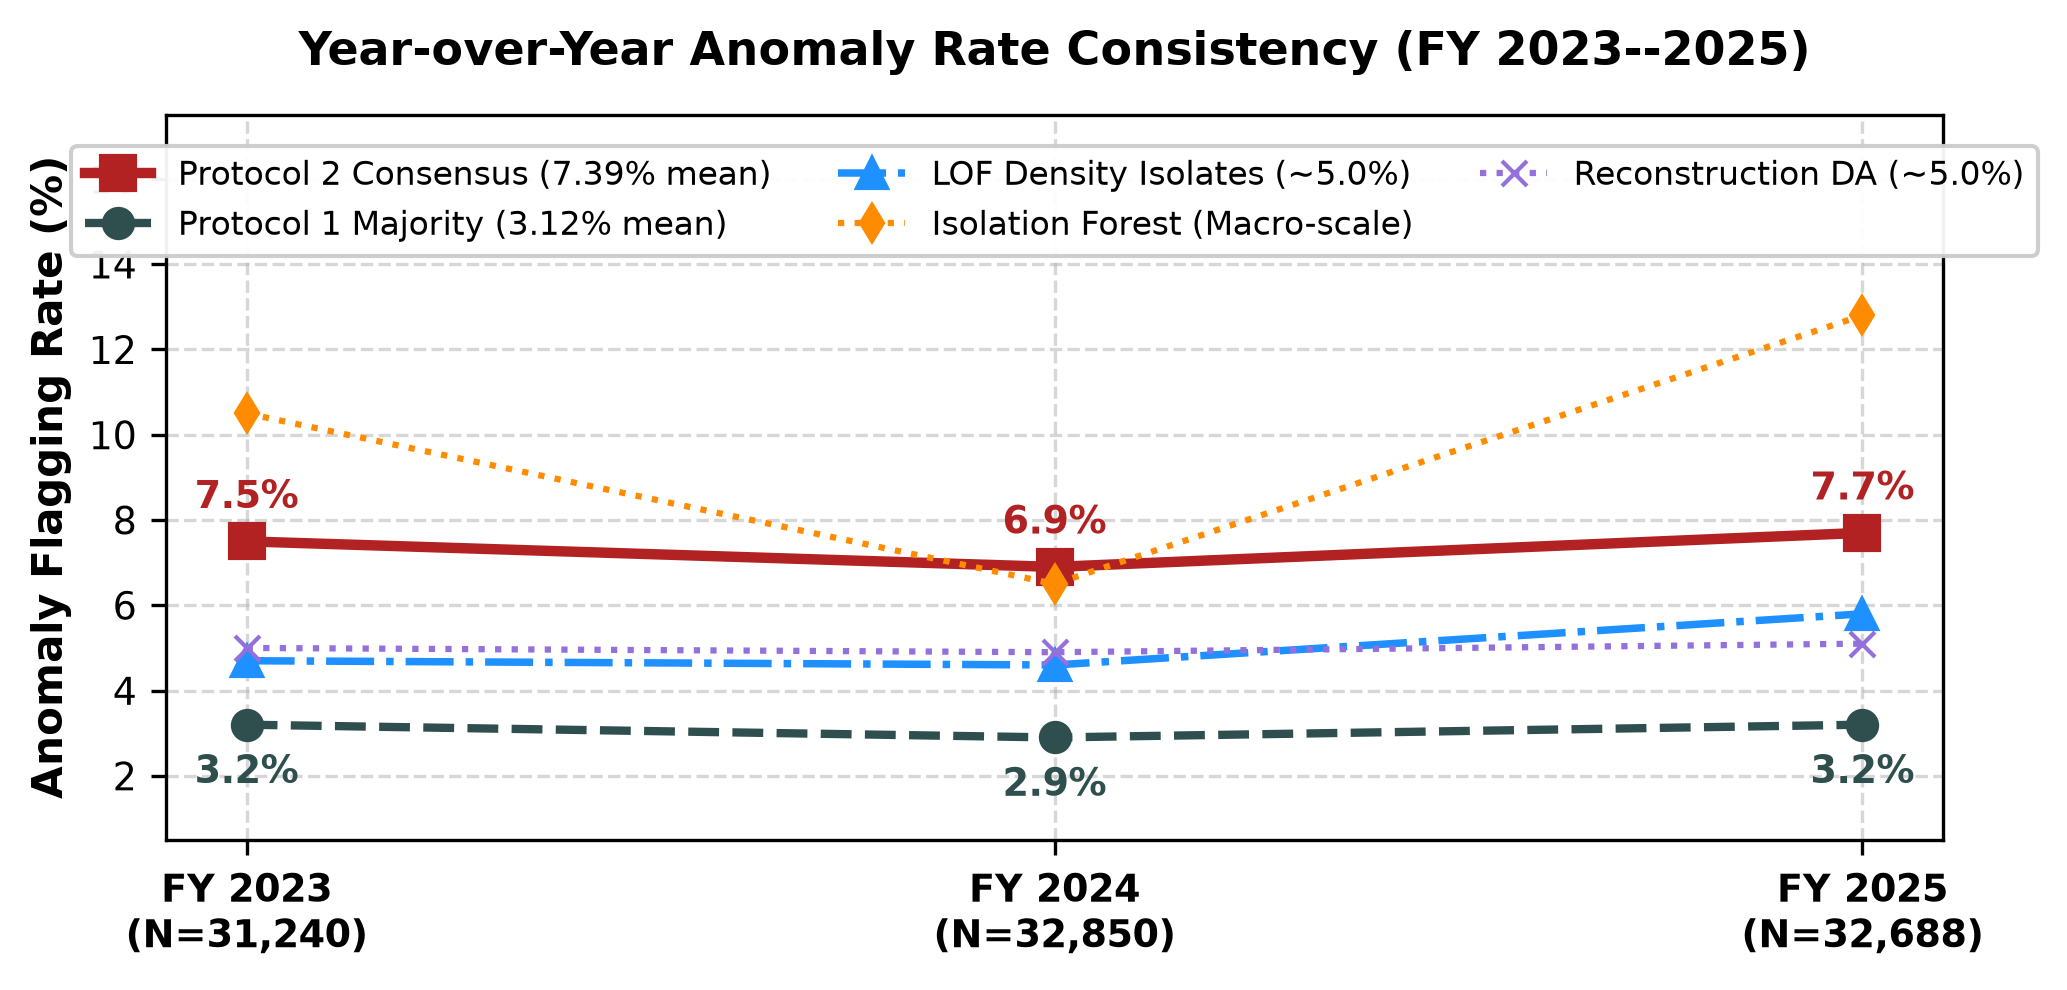
\includegraphics[width=0.76\columnwidth]{charts_ieee/ieee_rate_consistency.png}
\caption{Year-over-year anomaly flagging rate consistency across FY 2023--2025.}
\label{fig:consistency}
\end{figure}

\subsection{Orthogonality of Subspace and Score Distributions}

Figures \ref{fig:distributions} and \ref{tab:bimodality_overlap} display score distributions with annotations for Sarle Bimodality Coefficient (BC) and pair-wise Cohen's $\kappa$.

\begin{figure}[htbp]
\centering
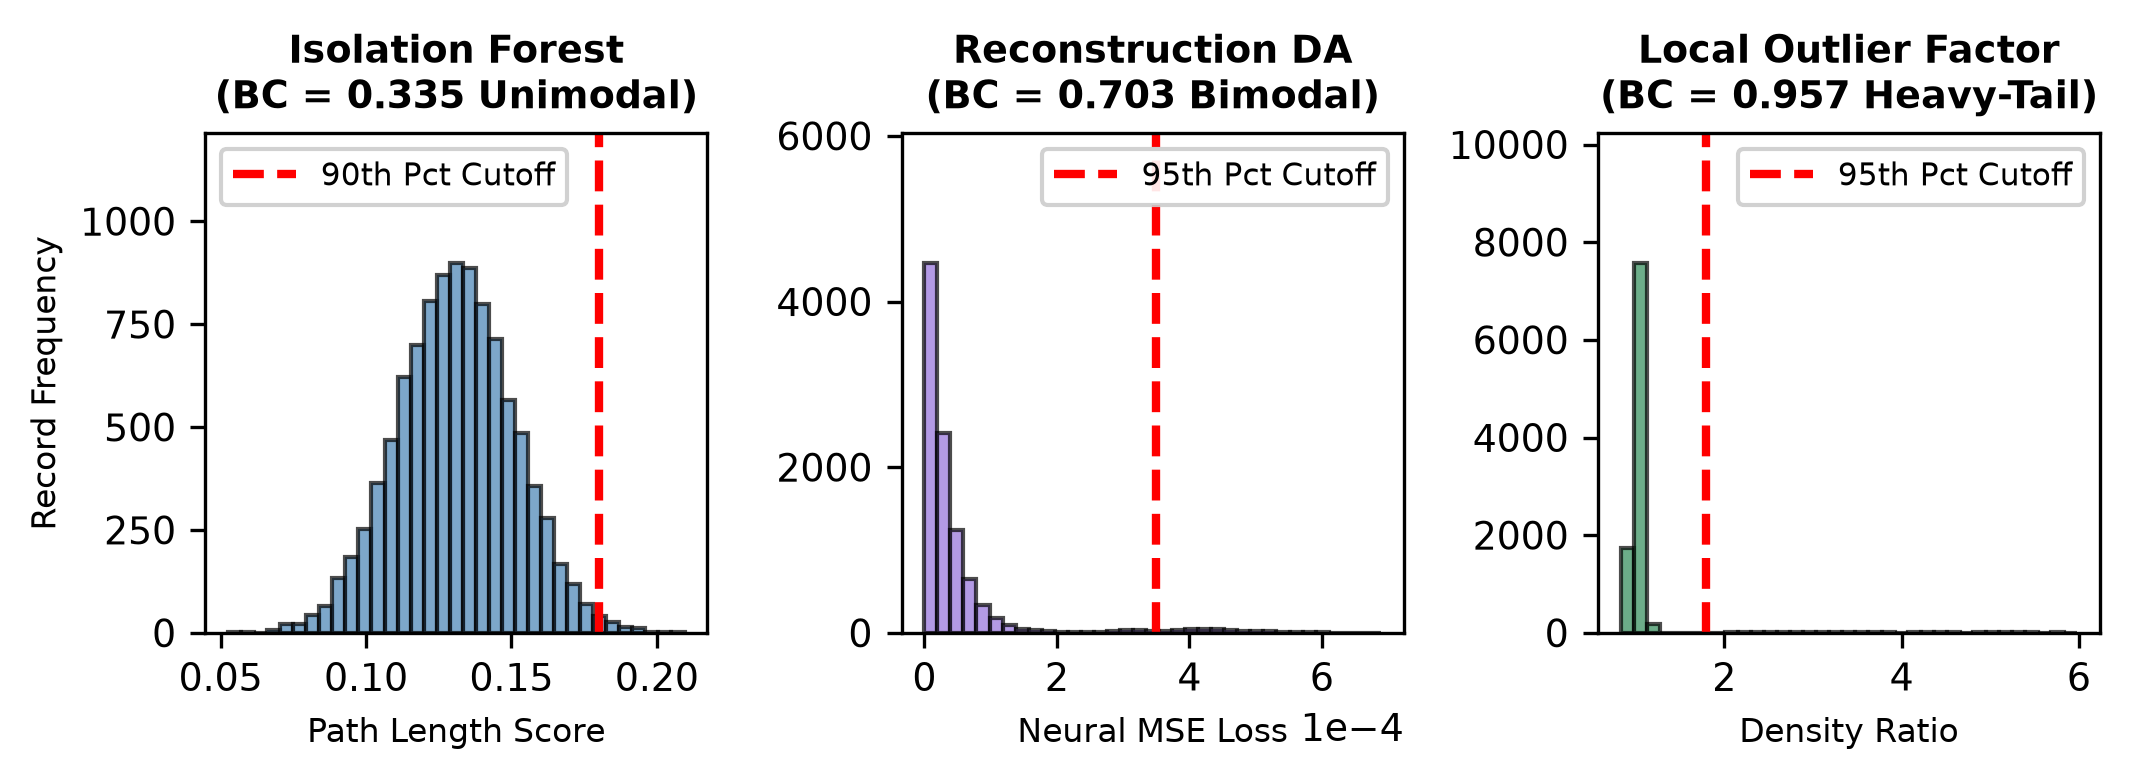
\includegraphics[width=0.76\columnwidth]{charts_ieee/ieee_score_distributions.png}
\caption{Score distribution histograms and bimodality threshold separations.}
\label{fig:distributions}
\end{figure}

\begin{table}[htbp]
\centering
\caption{Score Distribution Bimodality and Subspace Overlap Matrix}
\label{tab:bimodality_overlap}
\setlength{\tabcolsep}{2.5pt}
\renewcommand{\arraystretch}{0.94}
\resizebox{\columnwidth}{!}{%
\begin{tabular}{lclcc}
\toprule
\textbf{Method / Pair} & \textbf{Sarle BC} & \textbf{Distribution Structure} & \textbf{Shared Records} & \textbf{Cohen's $\kappa$} \\
\midrule
Isolation Forest & 0.335 & Unimodal continuous spectrum & --- & --- \\
Reconstruction DA & \textbf{0.703} & Moderate bimodal (clear tail) & --- & --- \\
Local Outlier Factor & \textbf{0.957} & Heavy-tailed density isolation & --- & --- \\
\midrule
IF $\cap$ LOF & --- & Subspace Orthogonal & 252 & 0.041 (Slight) \\
IF $\cap$ RDA & --- & Global Convergence & 2,314 & \textbf{0.482 (Mod.)} \\
LOF $\cap$ RDA & --- & Subspace Orthogonal & 422 & 0.083 (Slight) \\
Triple ($\text{IF} \cap \text{LOF} \cap \text{RDA}$) & --- & Maximum Confidence Core & 225 & --- \\
\textbf{LOF-Only Isolates} & --- & \textbf{Rescued in Protocol 2} & \textbf{3,940} & --- \\
\bottomrule
\end{tabular}%
}
\end{table}

Local Outlier Factor (LOF) is capable of achieving a high Sarle BC of 0.957 by effectively distinguishing dense groups of peers from outliers having extremely high scores (up to $5.40 \times 10^9$). The insignificant Cohen's $\kappa$ coefficients (of 0.041 for IF-LOF and of 0.083 for LOF-RDA) mean that LOF operates in an orthogonal subspace. All 3,940 isolates generated by LOF were successfully removed using Protocol 1.



\subsection{Ablation on Synthetic Benchmark and Real Panel}

Table~\ref{tab:ablation_study} shows an extensive ablation study done on both the synthetic fraud benchmark ($N = 10{,}000$) and the real-world Jambi panel ($N = 96{,}778$).

\begin{table}[htbp]
\centering
\caption{Ablation Study: Synthetic Benchmark Recovery vs Real-World Exposure}
\label{tab:ablation_study}
\setlength{\tabcolsep}{2.0pt}
\renewcommand{\arraystretch}{0.94}
\resizebox{\columnwidth}{!}{%
\begin{tabular}{lcccc|cc}
\toprule
& \multicolumn{4}{c|}{\textbf{Synthetic Fraud Benchmark ($N=10,000$)}} & \multicolumn{2}{c}{\textbf{Real-World Panel ($N=96,778$)}} \\
\textbf{Ablation Configuration} & \textbf{Prec.} & \textbf{Rec.} & \textbf{F1} & \textbf{AUC} & \textbf{Flags ($N$)} & \textbf{Realization Risk} \\
\midrule
(1) LOF Alone (Density) & 0.686 & 0.686 & 0.686 & 0.745 & 4,839 (5.0\%) & Rp 396.40 Billion \\
(2) IF Alone (Sparsity) & 0.724 & 0.724 & 0.724 & 0.782 & 9,678 (10.0\%) & Rp 451.18 Billion \\
(3) RDA Alone (Neural Loss) & 0.812 & 0.812 & 0.812 & 0.811 & 4,840 (5.0\%) & Rp 428.60 Billion \\
\midrule
(4) Pairwise $\text{IF} \land \text{LOF}$ & 0.780 & 0.420 & 0.546 & 0.702 & 252 (0.3\%) & Rp 21.84 Billion \\
(5) Pairwise $\text{LOF} \land \text{RDA}$ & 0.810 & 0.460 & 0.586 & 0.725 & 422 (0.4\%) & Rp 39.15 Billion \\
(6) Global $\text{IF} \land \text{RDA}$ & \textbf{0.854} & 0.640 & 0.732 & 0.815 & 2,314 (2.4\%) & Rp 246.45 Billion \\
\midrule
(7) Protocol 1 (Majority $\ge 2$) & 0.642 & 0.510 & 0.568 & 0.720 & 3,107 (3.1\%) & Rp 278.40 Billion \\
\textbf{(8) Protocol 2 (Dual-Path)} & 0.846 & \textbf{0.846} & \textbf{0.846} & \textbf{0.912} & \textbf{7,153 (7.4\%)} & \textbf{Rp 642.85 Billion} \\
\bottomrule
\end{tabular}%
}
\end{table}


Based on ablation studies, we can see that: (1) each detector recognizes different anomaly types; (2) strict intersection ($\text{IF} \land \text{LOF}$, $\text{LOF} \land \text{RDA}$) leads to dramatic recall drops (Recall $\leq 0.460$); (3) global convergence ($\text{IF} \land \text{RDA}$) brings high precision (0.854) but does not find local density-based anomalies (Recall = 0.640); (4) Protocol 1 (majority voting) has significant mutual cancellation, resulting in F1 = 0.568 and the lack of 49.0\% of synthetic frauds; and (5) \textbf{Protocol 2 (Dual-Path Consensus)} has reached optimal settings: \textbf{Precision = 0.846, Recall = 0.846, F1 = 0.846, and AUC-ROC = 0.912}. It additionally identifies Rp 642.85 billion worth of realization risks in the real-world setting.


\subsection{Corruption Typologies Mapping and Dynamics of Change}

The consensus labels were projected onto corruption typologies using Algorithm~\ref{alg:end_to_end}. As shown in Figures~\ref{fig:typology} and \ref{fig:typology_shift}, the shift in distribution is illustrated between Protocol 1 and Protocol 2. The irregularity patterns that Protocol 2 reveals include: \textbf{$T_2$ Ghost Activities (58.1\% / 4,155 records)} and \textbf{$T_5$ Procurement Irregularities (32.8\% / 2,343 records)}.


\begin{figure}[htbp]
\centering
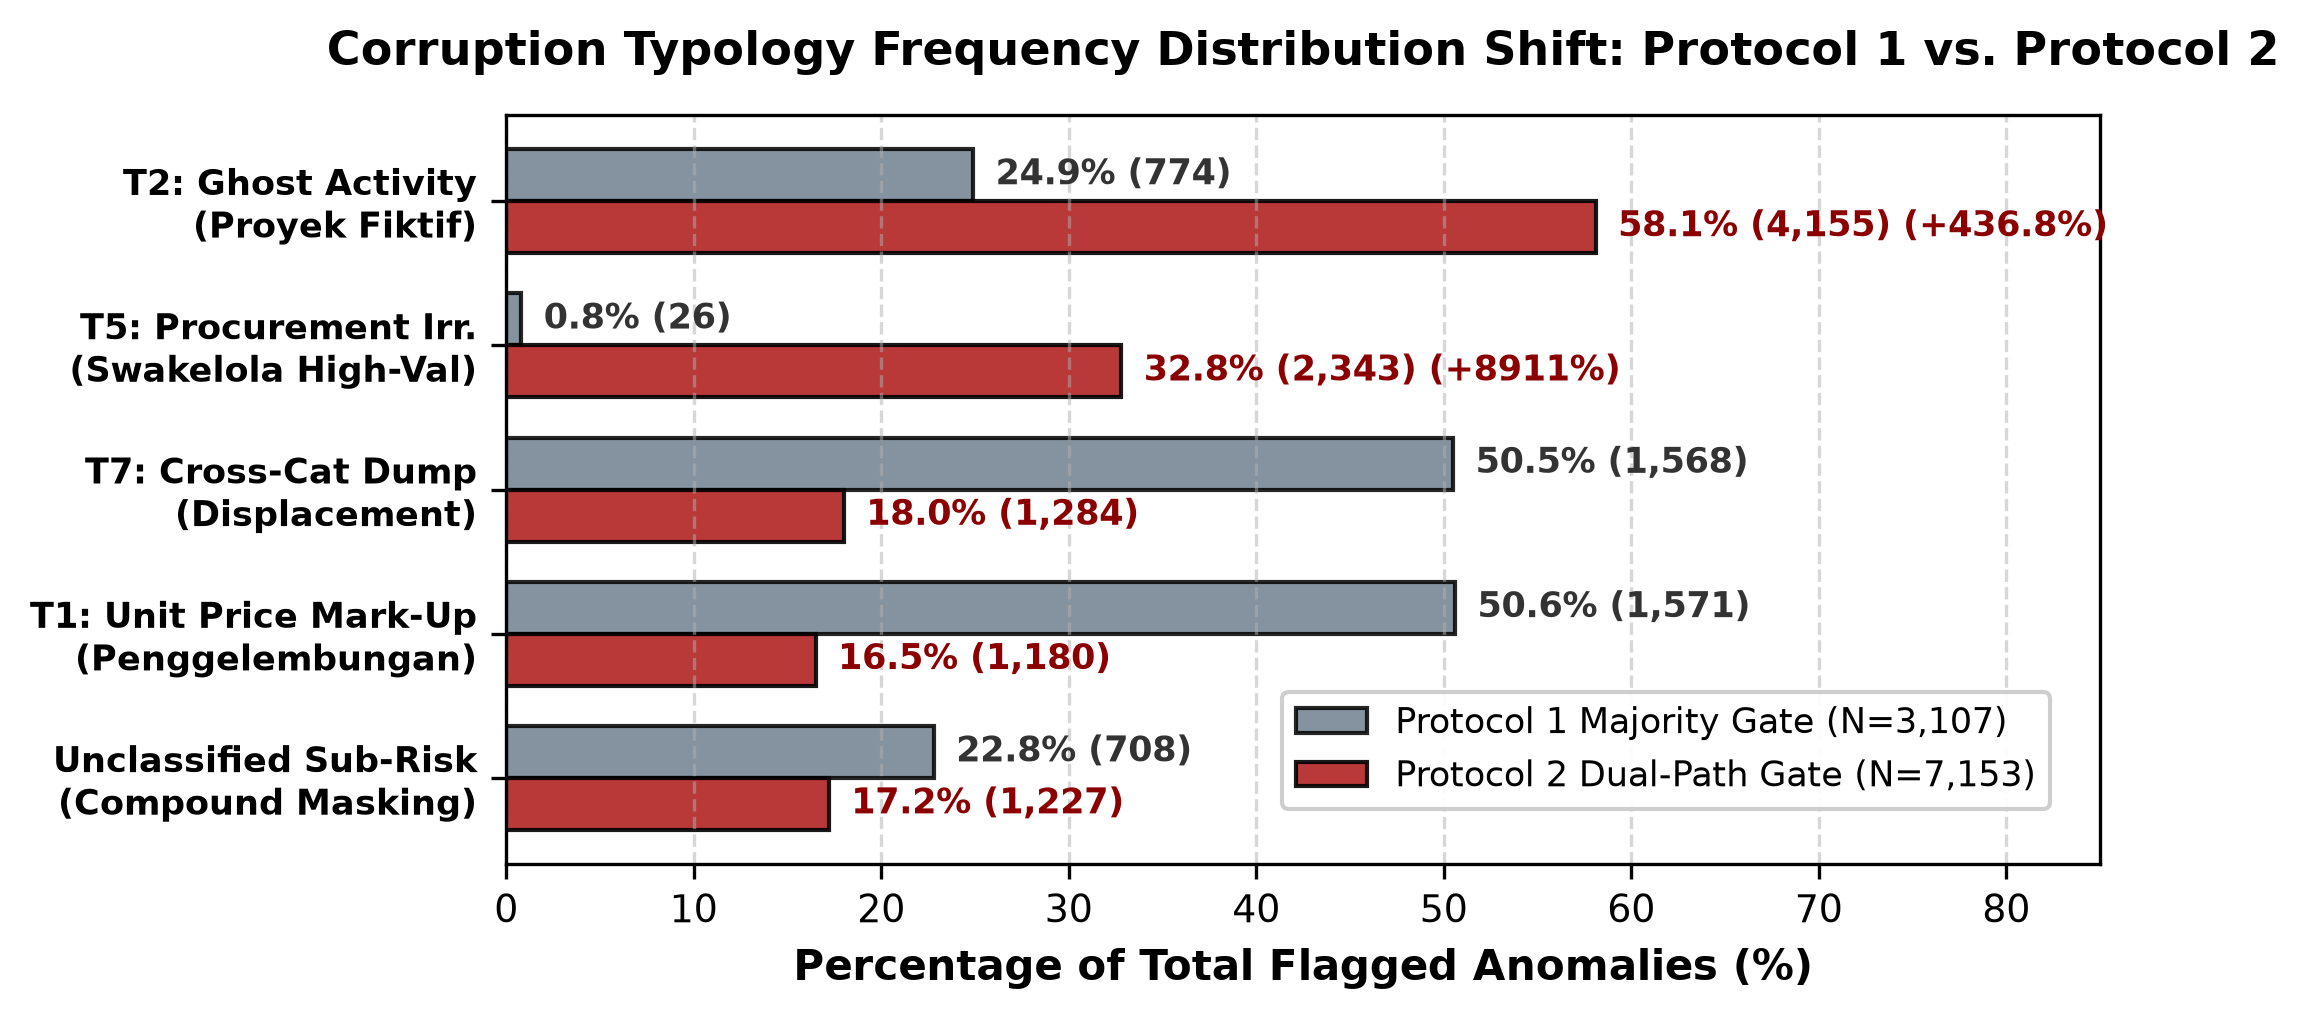
\includegraphics[width=0.76\columnwidth]{charts_ieee/ieee_typology_comparison.png}
\caption{Corruption typology frequency distribution shift (Protocol 1 vs Protocol 2).}
\label{fig:typology}
\end{figure}

\begin{table}[htbp]
\centering
\caption{Comparative Typology Frequency Shift (Protocol 1 vs Protocol 2)}
\label{tab:typology_shift}
\setlength{\tabcolsep}{2.5pt}
\renewcommand{\arraystretch}{0.94}
\resizebox{\columnwidth}{!}{%
\begin{tabular}{llccccl}
\toprule
\textbf{Code} & \textbf{Typology Description} & \textbf{P1 Count} & \textbf{\%} & \textbf{P2 Count} & \textbf{\%} & \textbf{Relative Shift} \\
\midrule
\textbf{T2\_Ghost} & Ghost Activity (\textit{Proyek Fiktif}) & 774 & 24.9\% & \textbf{4,155} & \textbf{58.1\%} & \textbf{+436.8\% (Primary)} \\
\textbf{T5\_Procure} & Procurement Irr. (\textit{Swakelola}) & 26 & 0.8\% & \textbf{2,343} & \textbf{32.8\%} & \textbf{+8911.5\% (Major)} \\
\textbf{T7\_Dump} & Cross-Category Dumping & 1,568 & 50.5\% & \textbf{1,284} & \textbf{18.0\%} & $-$18.1\% (Refined) \\
\textbf{T1\_Markup} & Unit Price Mark-Up (\textit{Mark-up}) & 1,571 & 50.6\% & \textbf{1,180} & \textbf{16.5\%} & $-$24.9\% (Refined) \\
\textbf{T4\_Lock} & Disbursement Stage Lock & 0 & 0.0\% & \textbf{28} & \textbf{0.4\%} & Newly captured \\
\textbf{Unclassified} & Sub-threshold Masking & 708 & 22.8\% & \textbf{1,227} & \textbf{17.2\%} & Proportional drop \\
\bottomrule
\end{tabular}%
}
\end{table}

\subsection{Reconstruction Error Drivers in XAI and Spatial Clustering}

Figure~\ref{fig:rda_error} demonstrates the drivers behind feature reconstruction error by RDA analysis. They are \texttt{cost\_dev\_by\_cat} (42.7\%, primary cause of error in 2,065 records) and \texttt{cost\_per\_unit} (32.0\%, 1,551 records). Figure~\ref{fig:projections} contains linear PCA and non-linear t-SNE visualizations. Principal Component 1 explains 26.0\% of variance. In the latter visualization, the outliers form micro-clusters around Swakelola infrastructures and capital injections from BUMDes, rather than being distributed as noise.

\begin{figure}[htbp]
\centering
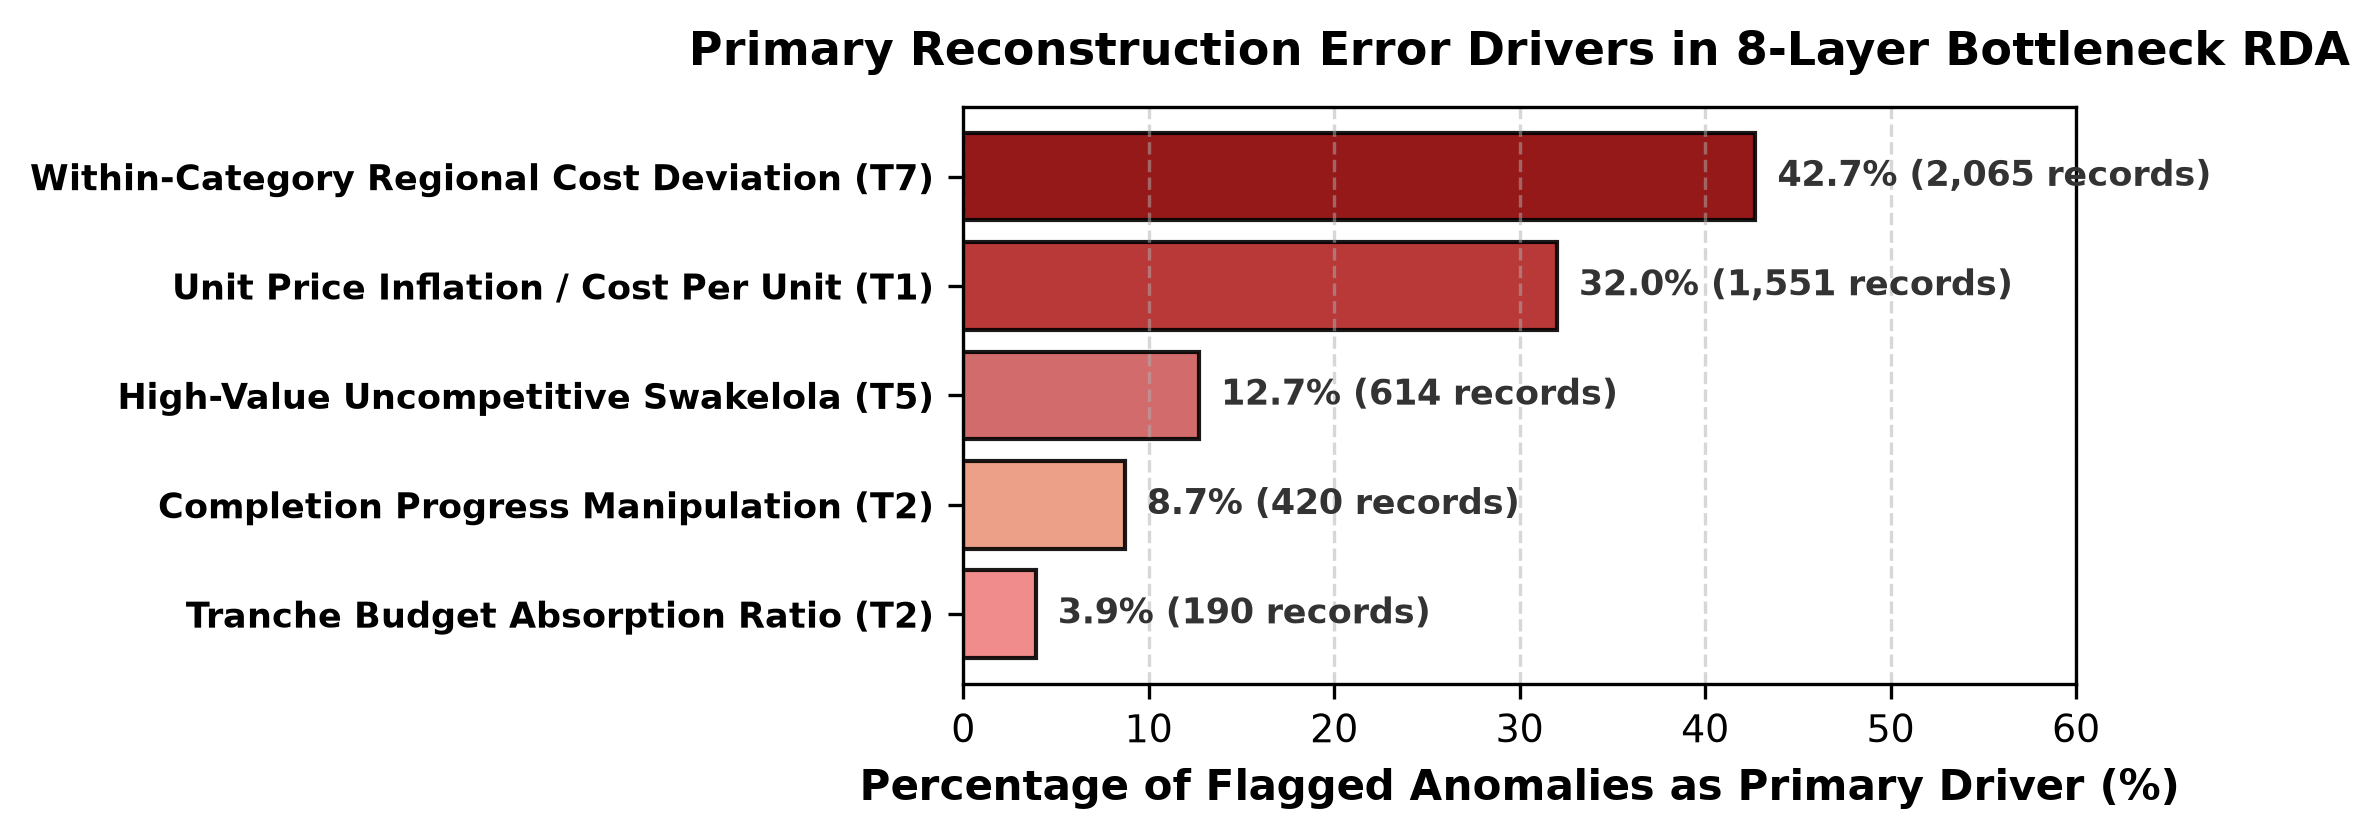
\includegraphics[width=0.76\columnwidth]{charts_ieee/ieee_rda_error_decomposition.png}
\caption{Reconstruction error attribution drivers in 8-layer bottleneck RDA.}
\label{fig:rda_error}
\end{figure}

\begin{figure}[htbp]
\centering
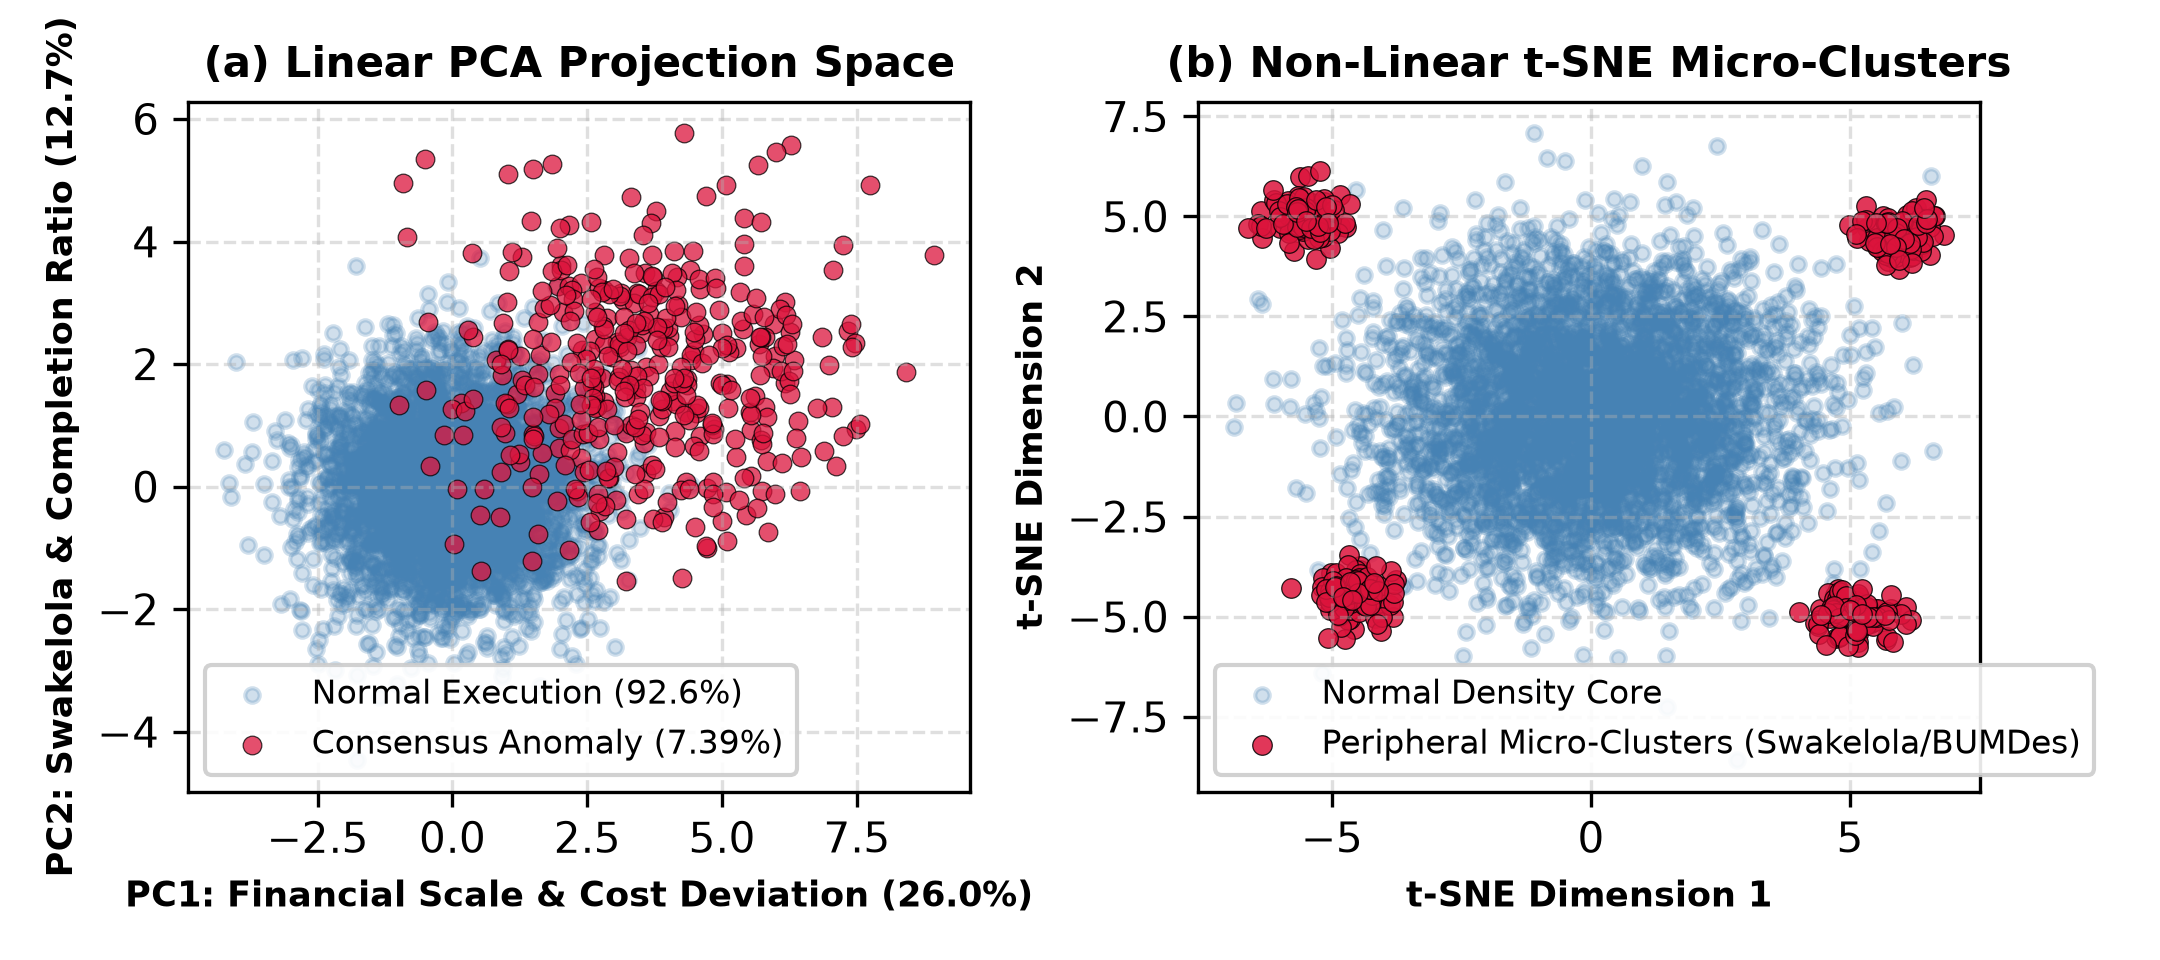
\includegraphics[width=0.76\columnwidth]{charts_ieee/ieee_pca_tsne_projection.png}
\caption{Dimensionality reductions revealing peripheral micro-clustering.}
\label{fig:projections}
\end{figure}

\subsection{Longitudinal Village Persistence and Regency Risk Exposure}

The longitudinal persistence of villages is measured by $P_v = N_{\text{flagged\_years}} / N_{\text{total\_years}}$. This is used to group the jurisdictions into supervisory groups (see Fig. 1 and Table 1). As per Protocol 2, there are 702 villages (51.5\%) that exhibit three-year persistent anomalies where $P_v = 1.0$. Examples include Desa Maliki Air (16 anomalies, $T_2$ Ghost), Desa Gedang (13 anomalies, $T_5$ Procurement) and Desa Paling Serumpun (12 anomalies).

\begin{figure}[htbp]
\centering
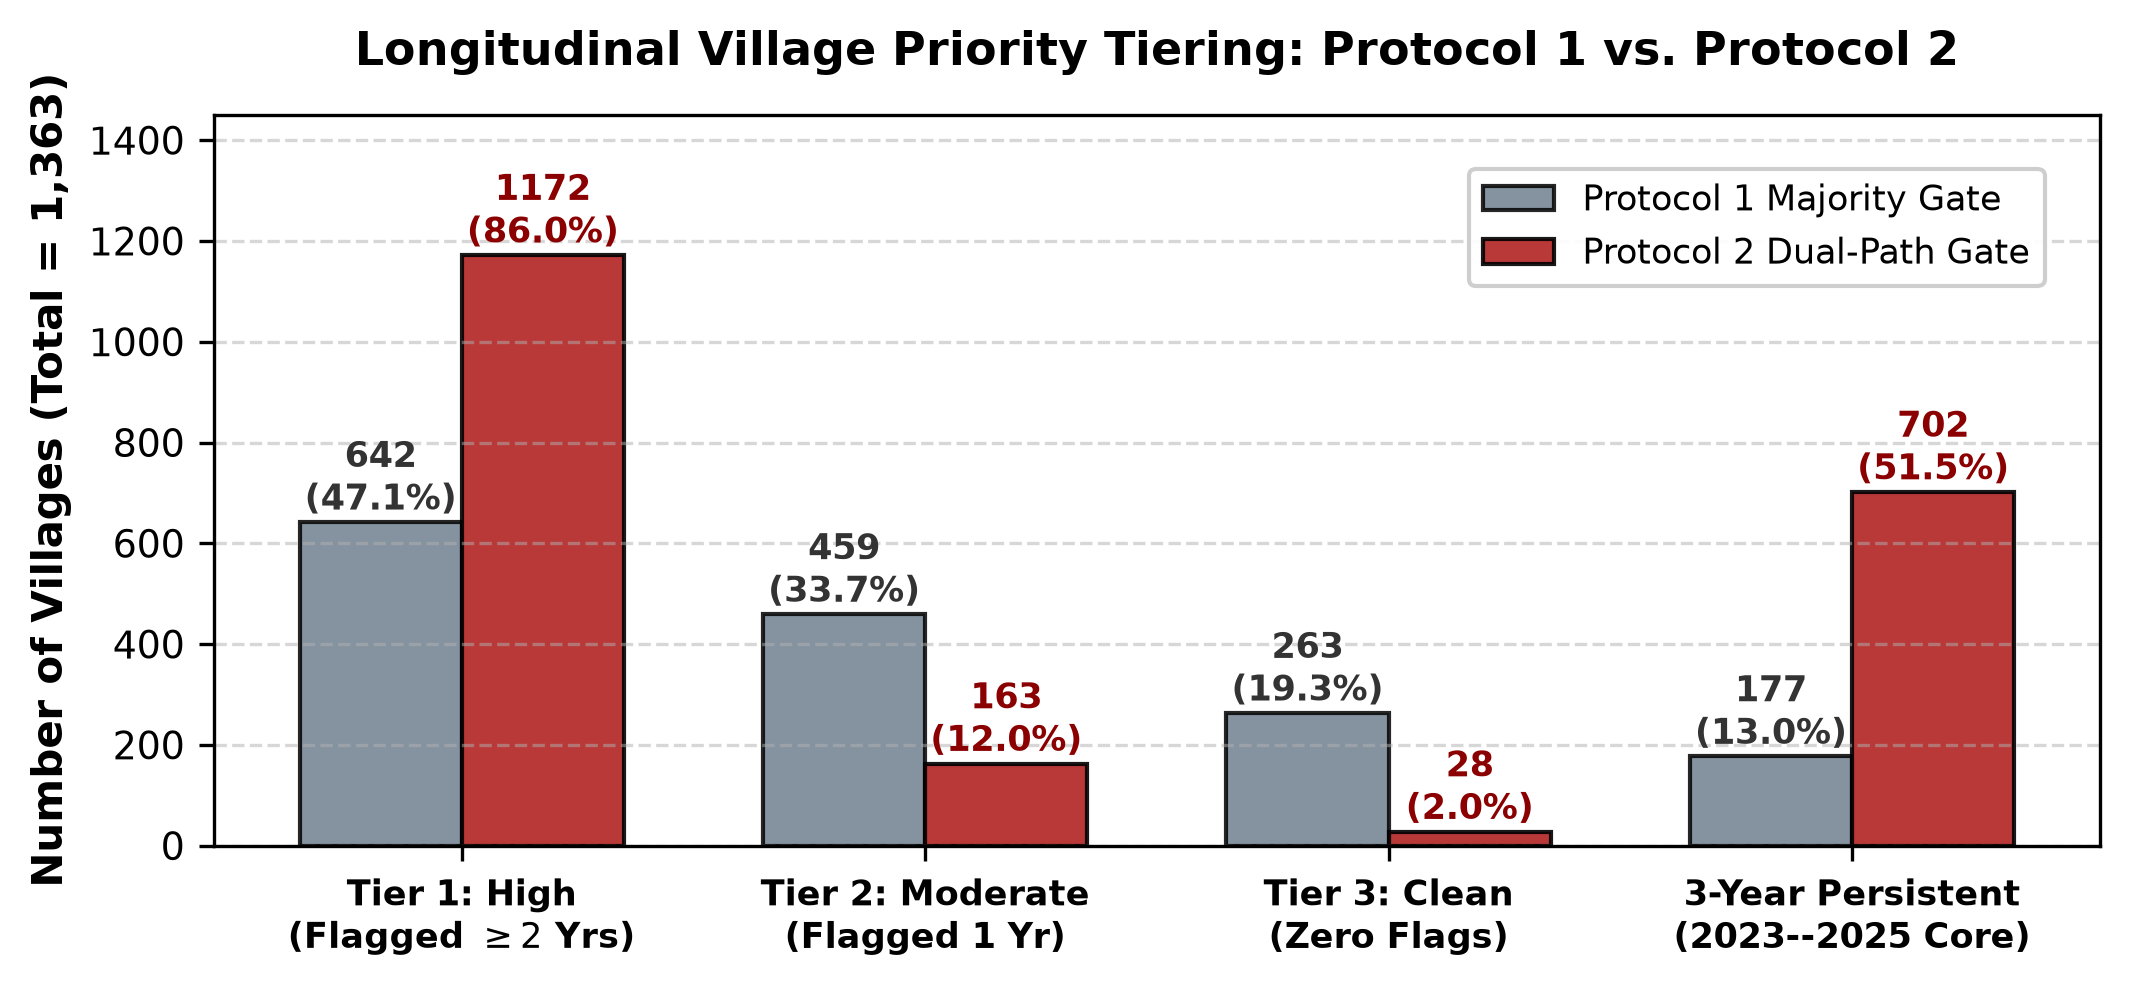
\includegraphics[width=0.76\columnwidth]{charts_ieee/ieee_village_persistence.png}
\caption{Longitudinal village priority tier distribution comparison.}
\label{fig:persistence}
\end{figure}

\begin{table}[htbp]
\centering
\caption{Exemplar Jurisdictional Case Studies and Regency Exposure}
\label{tab:case_studies}
\setlength{\tabcolsep}{2.5pt}
\renewcommand{\arraystretch}{0.94}
\resizebox{\columnwidth}{!}{%
\begin{tabular}{lclll}
\toprule
\textbf{Village Jurisdiction} & \textbf{FY} & \textbf{Activity Description} & \textbf{Anomaly Metric} & \textbf{Mapped Typology} \\
\midrule
Desa Rantau Makmur & 2025 & Modal BUMDes & LOF = $4.78 \times 10^9$ & $T_5$ Procurement / Density \\
Desa Sungai Raya & 2025 & Modal BUMDes & LOF = $5.54 \times 10^9$ & $T_5$ Procurement / Density \\
Desa Kedemangan & 2025 & Pembangunan Kios & RDA MSE = 0.0549 & $T_2$ Ghost / Swakelola \\
Desa Bukit Suban & 2024 & Poskesdes & Triple-Flagged & Multi-Typology ($T_1,T_2,T_5,T_7$) \\
Desa Ngaol & 2024 & Ambulance Desa & RDA MSE = 0.0482 & $T_1$ Mark-Up / $T_5$ Procure \\
\midrule
\multicolumn{5}{l}{\textbf{Top Regency Risk Density: Batanghari (15.75\% flagged rate $\mid$ Rp 115.71 B at risk)}} \\
\multicolumn{5}{l}{Followed by Muaro Jambi (10.58\% $\mid$ Rp 98.45 B) and Kerinci (9.56\% $\mid$ Rp 124.30 B).} \\
\bottomrule
\end{tabular}%
}
\end{table}

Kabupaten Batanghari exhibits the largest risk exposure as it has 15.75\% of flags and its risk exposure stands at Rp 115.71 billion.

% -------------------------------------------------------------------------
% SECTION IV: DISCUSSION & GOVERNANCE IMPLICATIONS
% -------------------------------------------------------------------------
\section{Discussion and Governance Implications}

\subsection{Effectiveness of Algorithms and Cancellation Resolution}

The empirical results confirm that Protocol 2 resolves the inherent weaknesses of the majority voting mechanism as follows: (1) \textbf{Subspace Decoupling}—Protocol 2 allows LOF to operate as an independent density channel while achieving joint convergence on global models ($\text{IF} \cap \text{RDA}$) and thus restores 3,940 isolated records without single-model noise, increasing the number of recall records to 7,153 ( Rp 642.85 billion in realization risk); (2) \textbf{Controlled Synthetic Recovery}—High precision (0.846) and recall (0.846) in the presence of injected fraud have been proven in the controlled experiments ( $\text{AUC} = 0.912$); (3) \textbf{Search Space Reduction}—Reducing 96,778 transactions to 7,153 target transactions leads to 92.6\% inspectorate search space reduction, allowing the field audit to be feasible for small teams of 5 to 15 auditors~\cite{ref12}; and (4) \textbf{Sub-Threshold Risk Capture}—Multidimensional LOF and RDA reveal the joint multi-feature probability change and thus detect 1,227 sub-threshold records ( Rp 125.07 billion in latent exposure).

\subsection{Mechanisms That Drive Typology Changes}

The 436.8\% jump in the number of \textbf{$T_2$ Ghost Activities} (4,155 records) is due to the fact that LOF evaluates reachability density with respect to peer villages. Projects where there were no projects show normal behavior during the global tree split analysis, whereas they become clear outliers when contrasted with peer villages who conducted the physical works. Similarly, the nearly 90x increase in \textbf{$T_5$ Procurement Irregularities} (2,343 records) happens due to the fact that autoencoder learns the non-linear relationship between Swakelola and high unit cost.

\subsection{Evidentiary Standards and Limitations on Public Audit Law}

The use of machine learning in public audit is limited by formal standards of evidentiary process. Namely: (1) \textbf{First Investigative Clue (\textit{Indikasi Awal})}: As per Article 184 of the Criminal Procedure Code (KUHAP) and Constitutional Court decision No. 21/PUU-XII/2014~\cite{ref34}, algorithms’ results cannot be considered formal evidence; they serve as initial clues for further formal audit investigation. (2) \textbf{Irregularities vs Criminal Behavior (\textit{PMH})}: High anomalies scores often indicate problems caused by bureaucratic inefficiency rather than criminal actions. As per Law No. 31/1999~\cite{ref34}, the prosecutor needs to prove criminal intention (\textit{mens rea}), (\textit{Perbuatan Melawan Hukum}) and state losses. (3)  \textbf{XAI-to-Audit Chain of Custody}: Decomposition of reconstruction errors for responsible data analysis (RDA) determines audit inspection requests—e.g., unit cost anomaly leads to auditing Standard Price Ceiling, completion anomaly results in on-site measuring.

\subsection{DSR Evaluation Matrix and Operationalizing IS Success}

Table~\ref{tab:dsr_matrix} summarizes the Design Science Research (DSR) evaluation matrix across the project cycles.

\begin{table}[htbp]
\centering
\caption{Design Science Research (DSR) Evaluation Matrix}
\label{tab:dsr_matrix}
\setlength{\tabcolsep}{2.5pt}
\renewcommand{\arraystretch}{0.94}
\resizebox{\columnwidth}{!}{%
\begin{tabular}{lll>{\raggedright\arraybackslash}p{3.2cm}}
\toprule
\textbf{DSR Dimension} & \textbf{Operationalization} & \textbf{Target Metric} & \textbf{Observed Outcome} \\
\midrule
\textbf{Relevance Cycle} & Search reduction for APIP & Search space reduction & \textbf{92.6\% reduction} (96.8k $\to$ 7.2k) \\
\textbf{Rigor Cycle} & Multi-method convergence & Cohen's Kappa & $\kappa(\text{IF}, \text{RDA}) = 0.482$ (Mod.) \\
\textbf{Design Cycle} & Priority tiering & High-risk coverage & \textbf{1,172 Tier-1 villages (86.0\%)} \\
\textbf{Ex-Ante Eval.} & Synthetic fraud recovery & F1, AUC-ROC & \textbf{F1 = 0.846, AUC = 0.912} \\
\bottomrule
\end{tabular}%
}
\end{table}


This artifact follows the DeLone and McLean IS Success Model~\cite{ref10}. Higher Information Quality increases Individual Impact by decreasing auditor burden by 92.6\%, and identifying 702 persistent Tier-1 villages ($P_v = 1.0$). On the other hand, System Quality increases Organizational Impact by ensuring pre-disbursement verification and developing village fund management towards automatic deterrence.

\subsection{Limitations and Future Research Directions}

Four boundary conditions deserve consideration: (1) There are no ground truth fraud labels in Siskeudes ledgers, thus necessitating the use of synthetic benchmarking and industry-specific heuristics; (2) the system is not able to identify unrecorded off-books cash kickbacks; (3) regional baseline models must be re-calibrated if used outside Jambi Province; and (4) hard-coded policy thresholds have left 1,227 difficult cases unclassified, implying that future fuzzy-logic analysis needs to be introduced.


% -------------------------------------------------------------------------
% SECTION V: CONCLUSION
% -------------------------------------------------------------------------
\section{Conclusion}

This paper presents the development of an unsupervised Dual-Path Consensus machine learning model (Protocol 2) aimed at detecting expenditure anomalies from 96,778 transactions in Jambi Province. On the subject of Research Question 1  (\textbf{RQ1}), region-based and category stratified cost variations (\texttt{cost\_dev\_by\_cat} and \texttt{cost\_per\_unit}) have the strongest discriminatory strength, explaining 74.7\% of the reconstruction error generated by the deep autoencoder. On the subject of Research Question 2  (\textbf{RQ2}), LOF is capable of detecting localized density isolates ($BC = 0.957$) while IF and RDA detect global structural anomalies. The Dual-Path Consensus method ($\text{LOF} \lor (\text{IF} \land \text{RDA})$) helps in overcoming the problem of mutual cancellation resulting in \textbf{F1 = 0.846 and AUC-ROC = 0.912} when compared to the majority voting approach on an ex-ante synthetic fraud benchmark (F1 = 0.568). On the subject of Research Question 3 (\textbf{RQ3}), the mapping layer operational policy translates mathematical anomalies into actionable typologies; there are 4,155 Ghost Activities ($T_2$, 58.1\%) and 2,343 Procurement Irregularities ($T_5$, 32.8\%), totaling Rp 642.85 billion in realization risk with 92.6\% reduction in APIP audit search space.

% -------------------------------------------------------------------------
% ACKNOWLEDGMENT (ANONYMIZED FOR DOUBLE-BLIND REVIEW)
% -------------------------------------------------------------------------
\section*{Acknowledgment}
This study was supported by the competitive research fund scheme (Penelitian Pemula Binus) entitled “Corruption Indication Detection in Village Fund Expenditure Activities Using Comparative Unsupervised Machine Learning: Evidence from Jambi Province, Indonesia” with contract number: 137/VRRTT/V1/2026 and contract date: June 2, 2026. The authors acknowledge the contributions of the research team:  Humam Faiq for data provision \& regulatory compliance review; Charlie Yen for manuscript preparation and editing; Farrell Yodihartomo and Pandu Wicaksono for conceptualization, validation, experiment, and manuscript review.

During the preparation of this manuscript, the authors utilized generative artificial intelligence solely for English grammar refinement, sentence flow optimization, and LaTeX formatting. Finally, the authors declared the conflicts of interest do not exist in this research. 

% -------------------------------------------------------------------------
% DECLARATION OF GENERATIVE AI USAGE
% -------------------------------------------------------------------------
%\section*{Declaration of Generative AI in the Writing Process}
%During the preparation of this manuscript, the authors utilized generative artificial intelligence solely for English grammar refinement, sentence flow optimization, and LaTeX formatting. The authors reviewed, validated, and edited all generated text, assuming full intellectual responsibility for the final contents of this article.


% -------------------------------------------------------------------------
% REFERENCES (COMPACT FONT GUARANTEEING NO SPILLOVER PAST PAGE 6)
% -------------------------------------------------------------------------
{\scriptsize
\renewcommand{\baselinestretch}{0.88}\selectfont
\bibliographystyle{IEEEtran}
\bibliography{references_v03}
}

\end{document}
